\documentclass[12pt,a4paper]{article}

% ─── Page Layout ───────────────────────────────────────────────────────────────
\usepackage[a4paper, margin=0.8in, headheight=14pt]{geometry}

% ─── Fonts (XeLaTeX) ───────────────────────────────────────────────────────────
\usepackage{fontspec}
\usepackage{unicode-math}
\setmainfont{TeX Gyre Pagella}
\setmonofont[Scale=0.88]{TeX Gyre Cursor}
\setmathfont{Latin Modern Math}

% ─── Packages ──────────────────────────────────────────────────────────────────
\usepackage{xcolor}
\usepackage{colortbl}
\usepackage{titlesec}
\usepackage{enumitem}
\usepackage{tabularx}
\usepackage{booktabs}
\usepackage{array}
\usepackage{amsmath}
\usepackage{tikz}
\usetikzlibrary{shapes.geometric, arrows.meta, positioning, calc, fit, decorations.pathreplacing}
\usepackage{tcolorbox}
\tcbuselibrary{skins, breakable}
\usepackage{hyperref}
\usepackage{fancyhdr}
\usepackage{graphicx}
\usepackage{microtype}
\hyphenpenalty=10000
\exhyphenpenalty=10000
\sloppy
\usepackage{caption}
\usepackage{setspace}
\usepackage{multirow}
\usepackage{tocloft}

% ─── Q&A helper ────────────────────────────────────────────────────────────────
\newcommand{\Q}[1]{\textbf{#1}\par\noindent\ignorespaces}

% ─── Colour Palette ────────────────────────────────────────────────────────────
\definecolor{myred}{RGB}{196,30,58}
\definecolor{mydark}{RGB}{30,30,50}
\definecolor{mygreen}{RGB}{14,120,80}
\definecolor{myteal}{RGB}{0,130,140}
\definecolor{myamber}{RGB}{180,100,0}
\definecolor{mypurple}{RGB}{100,30,160}
\definecolor{mygray}{RGB}{246,247,249}
\definecolor{mgframe}{RGB}{180,185,200}
\definecolor{watermark}{RGB}{145,150,170}
\definecolor{hdrred}{RGB}{250,232,235}
\definecolor{hdrgreen}{RGB}{220,244,233}
\definecolor{hdrteal}{RGB}{220,242,244}
\definecolor{hdramber}{RGB}{253,242,215}
\definecolor{hdrpurple}{RGB}{238,228,255}
\definecolor{hdrgray}{RGB}{238,240,245}
\definecolor{rowalt}{RGB}{250,251,253}

% ─── Section Formatting ────────────────────────────────────────────────────────
\titleformat{\section}
  {\large\bfseries\color{myred}}{\thesection.}{0.5em}{}
  [\vspace{1pt}{\color{myred}\rule{\linewidth}{0.8pt}}]
\titleformat{\subsection}
  {\normalsize\bfseries\color{myteal}}{\thesubsection}{0.5em}{}
\titlespacing*{\section}{0pt}{18pt}{7pt}
\titlespacing*{\subsection}{0pt}{11pt}{4pt}

% ─── Paragraph ─────────────────────────────────────────────────────────────────
\setlength{\parindent}{0pt}
\setlength{\parskip}{4pt}

% ─── TOC Styling ───────────────────────────────────────────────────────────────
\renewcommand{\cfttoctitlefont}{\large\bfseries\color{myred}}
\renewcommand{\cftaftertoctitle}{\par\noindent{\color{myred}\rule{\linewidth}{0.8pt}}}
\setlength{\cftbeforetoctitleskip}{0pt}
\setlength{\cftaftertoctitleskip}{6pt}
\renewcommand{\cftsecfont}{\normalsize\bfseries\color{mydark}}
\renewcommand{\cftsecpagefont}{\normalsize\bfseries\color{mydark}}
\renewcommand{\cftsecleader}{\cftdotfill{\cftdotsep}}
\setlength{\cftbeforesecskip}{7pt}
\renewcommand{\cftsubsecfont}{\small\color{mydark}}
\renewcommand{\cftsubsecpagefont}{\small\color{mydark}}
\setlength{\cftbeforesubsecskip}{3pt}
\setlength{\cftsubsecindent}{1.4em}

% ─── Table helpers ─────────────────────────────────────────────────────────────
\renewcommand{\arraystretch}{1.45}
\setlength{\tabcolsep}{6pt}
\arrayrulecolor{mydark}
\newcolumntype{B}[1]{>{\small\bfseries\raggedright\arraybackslash}m{#1}}
\newcolumntype{Y}{>{\small\raggedright\arraybackslash}X}
\renewcommand{\tabularxcolumn}[1]{m{#1}}

% ─── Header / Footer ───────────────────────────────────────────────────────────
\pagestyle{fancy}
\fancyhf{}
\fancyhead[L]{\small\color{myred}\textbf{PE-EC702B}\;\color{mydark}--- Digital Image and Video Processing}
\fancyhead[R]{\small\color{myteal}\textbf{Module 2 Notes}}
\fancyfoot[C]{\small\color{mydark}\thepage}
\fancyfoot[R]{\small\color{watermark}\textit{\copyright\ Biraj}}
\renewcommand{\headrulewidth}{0.5pt}
\renewcommand{\footrulewidth}{0.3pt}

% ─── Hyperref ──────────────────────────────────────────────────────────────────
\hypersetup{
  colorlinks=true, linkcolor=myteal, urlcolor=myteal,
  pdfauthor={Biraj Sarkar},
  pdftitle={PE-EC702B --- Module 2 Notes}
}

% ─── tcolorbox styles ──────────────────────────────────────────────────────────
\tcbset{
  tikzbox/.style={
    colback=mygray, colframe=mgframe, boxrule=0.6pt, arc=4pt,
    left=8pt, right=8pt, top=6pt, bottom=6pt,
    colbacktitle=mgframe, coltitle=mydark,
    fonttitle=\small\bfseries
  },
  defbox/.style={
    colback=hdrgreen, colframe=mygreen, boxrule=0.8pt, arc=4pt,
    left=9pt, right=9pt, top=6pt, bottom=6pt,
    colbacktitle=mygreen, coltitle=white,
    fonttitle=\small\bfseries
  },
  formulabox/.style={
    colback=hdrteal, colframe=myteal, boxrule=0.8pt, arc=4pt,
    left=9pt, right=9pt, top=7pt, bottom=7pt,
    colbacktitle=myteal, coltitle=white,
    fonttitle=\small\bfseries
  },
  examplebox/.style={
    colback=hdramber, colframe=myamber, boxrule=0.8pt, arc=4pt,
    left=9pt, right=9pt, top=6pt, bottom=6pt,
    colbacktitle=myamber, coltitle=white,
    fonttitle=\small\bfseries,
    breakable
  },
  masonbox/.style={
    colback=hdrpurple, colframe=mypurple, boxrule=0.8pt, arc=4pt,
    left=9pt, right=9pt, top=6pt, bottom=6pt,
    colbacktitle=mypurple, coltitle=white,
    fonttitle=\small\bfseries
  },
  exambox/.style={
    colback=hdrpurple, colframe=mypurple, boxrule=1pt, arc=5pt,
    left=10pt, right=10pt, top=8pt, bottom=8pt,
    colbacktitle=mypurple, coltitle=white,
    fonttitle=\bfseries,
    breakable, title after break={\textbf{Frequently Asked / Viva Questions (contd.)}}}
}
\tcbset{breakable}

% ─── TikZ styles ───────────────────────────────────────────────────────────────
\tikzset{
  block/.style={rectangle, draw=myteal, fill=hdrteal,
    text width=2.1cm, align=center, minimum height=0.85cm,
    font=\small, rounded corners=3pt, line width=0.7pt},
  arrow/.style={-Stealth, thick, color=mydark},
  line/.style={thick, color=mydark}
}

% ═══════════════════════════════════════════════════════════════════════════════
\begin{document}
% ═══════════════════════════════════════════════════════════════════════════════

\begin{center}
  {\LARGE\bfseries\color{myred} PE-EC702B --- Digital Image and Video Processing}\\[5pt]
  {\normalsize\color{mydark} Semester VII \quad$\bullet$\quad 3L:0T:0P \quad$\bullet$\quad 3 Credits}\\[3pt]
  {\normalsize\color{myteal}\textbf{Module 2 Exam Notes: Image Enhancements and Filtering}}\\[3pt]
  {\small\color{mydark} CGEC \;$|$\; B.Tech ECE (2023--27) \;$|$\; \textit{Biraj Sarkar}}
\end{center}
\vspace{2pt}
\noindent{\color{myred}\rule{\linewidth}{1.5pt}}
\vspace{2pt}

\hypersetup{linkcolor=mydark}
\tableofcontents
\hypersetup{linkcolor=myteal}
\newpage

% ===============================================================================
\section{Gray Level Transformations}
% ===============================================================================

Gray level transformations operate directly on individual pixel values in the spatial domain. The basic mapping function is $s = T(r)$, where $r$ is the input intensity and $s$ is the processed intensity.

\begin{tcolorbox}[defbox, title={Standard Gray Level Mapping Functions}]
\begin{enumerate}[label=\arabic*., leftmargin=*, itemsep=2.5pt]
  \item \textbf{Image Negatives:} Reverses the intensity levels of an image:
    \begin{equation}
      s = L - 1 - r
    \end{equation}
    where $L$ is the number of gray levels. Useful for enhancing white or light detail embedded in dark regions.
  \item \textbf{Log Transformations:} Expands dynamic range of dark pixels while compressing high-level values:
    \begin{equation}
      s = c \log(1 + r)
    \end{equation}
    where $c$ is a constant. Highly useful for displaying Fourier spectra that contain huge intensity ranges.
  \item \textbf{Power-Law (Gamma) Transformations:} Maps a narrow band of dark values into a wider range:
    \begin{equation}
      s = c r^\gamma
    \end{equation}
    where $\gamma$ is the exponent.
    \begin{itemize}[leftmargin=1em, itemsep=1pt]
      \item $\gamma < 1$: Expands dark regions, compresses bright regions.
      \item $\gamma > 1$: Compresses dark regions, expands bright regions.
    \end{itemize}
\end{enumerate}
\end{tcolorbox}

% ===============================================================================
\section{Histogram Processing}
% ===============================================================================

The histogram of a digital image with intensity levels in $[0, L-1]$ is a discrete function $h(r_k) = n_k$, where $n_k$ is the number of pixels with intensity $r_k$.

\subsection{Histogram Equalization}
Histogram equalization is an automated method to improve image contrast by transforming the intensity values such that the output image has a uniform distribution of gray levels.

\begin{tcolorbox}[formulabox, title={Continuous Case Derivation}]
Let $r$ be a continuous variable in $[0, L-1]$. We seek a transformation $s = T(r)$ satisfying:
\begin{enumerate}[label=(\roman*), leftmargin=*, itemsep=1pt]
  \item $T(r)$ is monotonically increasing (preserves intensity order).
  \item $0 \le T(r) \le L-1$ for $0 \le r \le L-1$.
\end{enumerate}
Using probability theory, the probability density function (PDF) of the transformed variable $s$, $p_s(s)$, is:
\begin{equation}
  p_s(s) = p_r(r) \left| \frac{dr}{ds} \right|
\end{equation}
Let us choose the transformation function to be the cumulative distribution function (CDF) of $r$:
\begin{equation}
  s = T(r) = (L-1) \int_0^r p_r(w) \, dw
\end{equation}
Differentiating $s$ with respect to $r$ using the Fundamental Theorem of Calculus:
\begin{equation}
  \frac{ds}{dr} = \frac{dT(r)}{dr} = (L-1) p_r(r)
\end{equation}
Substituting this back into the PDF expression:
\begin{equation}
  p_s(s) = p_r(r) \left| \frac{1}{(L-1) p_r(r)} \right| = \frac{1}{L-1}
\end{equation}
This proves that the resulting PDF $p_s(s)$ is flat (uniform) over the range $[0, L-1]$.
\end{tcolorbox}

For discrete images, the transformation function is:
\begin{equation}
  s_k = T(r_k) = (L-1) \sum_{j=0}^k p_r(r_j) = \frac{L-1}{MN} \sum_{j=0}^k n_j
\end{equation}
where $MN$ is the total number of pixels in the image.

\subsection{Histogram Specification}
Histogram specification allows us to designate the shape of the histogram we wish the processed image to have, rather than just generating a uniform histogram.
\begin{enumerate}[leftmargin=*, itemsep=2.5pt]
  \item Equalize the input image to get $s_k = T(r_k)$.
  \item Compute the transformation function $G(z_q)$ for the specified output histogram:
    \begin{equation}
      v_q = G(z_q) = (L-1)\sum_{i=0}^q p_z(z_i)
    \end{equation}
  \item Perform the inverse mapping: $z_q = G^{-1}(s_k)$.
\end{enumerate}

% ===============================================================================
\section{Spatial Domain Filtering}
% ===============================================================================

Spatial filtering involves moving a filter mask (kernel) over each pixel of an image to perform operations on the pixel neighborhood.

\subsection{Smoothing Filters (Low-pass)}
\begin{itemize}[leftmargin=*, itemsep=3.5pt]
  \item \textbf{Linear Smoothing Filters:} Replacing each pixel by the average of its neighbors (e.g., Box filter, Gaussian filter). Reduces noise but blurs edges.
  \item \textbf{Order-Statistics Filters (Non-linear):} Replacement based on ordering (ranking) the pixels in the neighborhood.
    \begin{itemize}[leftmargin=1.5em, itemsep=1.5pt]
      \item \textbf{Median Filter:} Replaces pixel value with the median of the neighborhood. Excellent for removing \textbf{salt-and-pepper (impulse) noise} while preserving edges.
      \item \textbf{Max/Min Filters:} Replaces with maximum/minimum value (enhances bright/dark details).
    \end{itemize}
\end{itemize}

\subsection{Sharpening Filters (High-pass)}
Sharpening highlights transitions in intensity (edges) using spatial differentiation.
\begin{enumerate}[leftmargin=*, itemsep=3.5pt]
  \item \textbf{First-Derivative Sharpening (Gradient):}
    The gradient magnitude is used to detect edges. The Sobel operator uses two $3 \times 3$ masks to compute horizontal ($G_x$) and vertical ($G_y$) gradients:
    \begin{equation}
      G_x = \begin{bmatrix} -1 & 0 & 1 \\ -2 & 0 & 2 \\ -1 & 0 & 1 \end{bmatrix}, \quad
      G_y = \begin{bmatrix} -1 & -2 & -1 \\ 0 & 0 & 0 \\ 1 & 2 & 1 \end{bmatrix}
    \end{equation}
  \item \textbf{Second-Derivative Sharpening (Laplacian):}
    The isotropic Laplacian operator is defined as:
    \begin{equation}
      \nabla^2 f = \frac{\partial^2 f}{\partial x^2} + \frac{\partial^2 f}{\partial y^2}
    \end{equation}
    The standard discrete Laplacian mask is:
    \begin{equation}
      H = \begin{bmatrix} 0 & 1 & 0 \\ 1 & -4 & 1 \\ 0 & 1 & 0 \end{bmatrix} \quad \text{or} \quad
      H_{\text{diag}} = \begin{bmatrix} 1 & 1 & 1 \\ 1 & -8 & 1 \\ 1 & 1 & 1 \end{bmatrix}
    \end{equation}
\end{enumerate}

% ===============================================================================
\section{Frequency Domain Filtering}
% ===============================================================================

Frequency filtering operates on the 2D Discrete Fourier Transform (DFT) of the image.

\begin{tcolorbox}[tikzbox, title={Spatial vs. Frequency Domain Filtering Flow}]
\centering
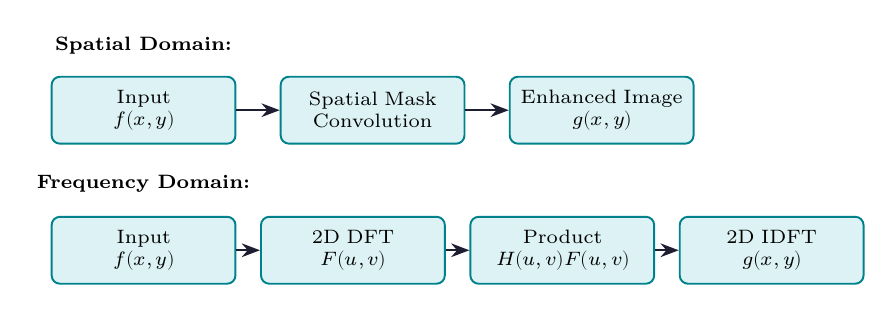
\begin{tikzpicture}[node distance=0.3cm and 0.55cm,
  sblock/.style={rectangle, draw=myteal, fill=hdrteal, text width=2.1cm,
    align=center, minimum height=0.85cm, font=\scriptsize,
    rounded corners=3pt, line width=0.7pt}]

  % Spatial Domain
  \node[font=\scriptsize\bfseries] (lbl1) at (0, 0.75) {Spatial Domain:};
  \node[sblock, below=0.15cm of lbl1] (s_in) {Input\\$f(x,y)$};
  \node[sblock, right=of s_in] (s_filt) {Spatial Mask\\Convolution};
  \node[sblock, right=of s_filt] (s_out) {Enhanced Image\\$g(x,y)$};
  \draw[arrow] (s_in) -- (s_filt);
  \draw[arrow] (s_filt) -- (s_out);

  % Frequency Domain
  \node[font=\scriptsize\bfseries] (lbl2) at (0, -1.0) {Frequency Domain:};
  \begin{scope}[shift={(0, -1.85)}]
    \node[sblock] (f_in) {Input\\$f(x,y)$};
    \node[sblock, right=0.3cm of f_in] (f_dft) {2D DFT\\$F(u,v)$};
    \node[sblock, right=0.3cm of f_dft] (f_mult) {Product\\$H(u,v)F(u,v)$};
    \node[sblock, right=0.3cm of f_mult] (f_idft) {2D IDFT\\$g(x,y)$};
    \draw[arrow] (f_in) -- (f_dft);
    \draw[arrow] (f_dft) -- (f_mult);
    \draw[arrow] (f_mult) -- (f_idft);
  \end{scope}
\end{tikzpicture}
\end{tcolorbox}

Let $D(u,v) = \sqrt{(u - M/2)^2 + (v - N/2)^2}$ be the distance from the center of the frequency rectangle.
\begin{itemize}[leftmargin=*, itemsep=3.5pt]
  \item \textbf{Low-Pass Filters (LPF):} Smooths images by attenuating high frequencies.
    \begin{itemize}[leftmargin=1.5em, itemsep=1.5pt]
      \item \textbf{Ideal LPF:} $H(u,v) = 1$ if $D(u,v) \le D_0$; else $0$. Introduces severe \textbf{ringing artifacts} due to sharp transition.
      \item \textbf{Butterworth LPF (order $n$):} $H(u,v) = \frac{1}{1 + [D(u,v)/D_0]^{2n}}$. Smooth transition, less ringing.
      \item \textbf{Gaussian LPF:} $H(u,v) = e^{-D^2(u,v)/2D_0^2}$. Completely free of ringing.
    \end{itemize}
  \item \textbf{High-Pass Filters (HPF):} Sharpens images (high frequencies are kept, low frequencies attenuated). Formulas are $H_{\text{HPF}}(u,v) = 1 - H_{\text{LPF}}(u,v)$.
\end{itemize}

% ===============================================================================
\section{Worked Examples}
% ===============================================================================

\begin{tcolorbox}[examplebox, title={Discrete Histogram Equalization}]
\textbf{Problem:} Equalize a 3-bit image ($L=8$ levels) of size $64 \times 64$ ($MN = 4096$) with the following gray-level distribution:
\begin{center}
  \small
  \begin{tabular}{c c c c c c c c c}
    \toprule
    Gray Level $r_k$ & 0 & 1 & 2 & 3 & 4 & 5 & 6 & 7 \\
    \midrule
    Pixel count $n_k$ & 790 & 1023 & 850 & 656 & 329 & 245 & 122 & 81 \\
    \bottomrule
  \end{tabular}
\end{center}

\par\noindent\rule{\linewidth}{0.5pt}\par
\textbf{Solution:}
We use the transformation formula: $s_k = \text{round}\left( (L-1) \sum_{j=0}^k \frac{n_j}{MN} \right) = \text{round}\left( \frac{7}{4096} \sum_{j=0}^k n_j \right)$.
Let's compute the cumulative sum and map the values step-by-step:

\begin{enumerate}[leftmargin=*, itemsep=3.5pt]
  \item \textbf{For $k=0$ ($r_0 = 0$):}
    Cumulative sum $\sum = 790$.
    $s_0 = \frac{7}{4096} \times 790 = 1.35 \rightarrow \text{round}(1.35) = 1$.
  \item \textbf{For $k=1$ ($r_1 = 1$):}
    Cumulative sum $\sum = 790 + 1023 = 1813$.
    $s_1 = \frac{7}{4096} \times 1813 = 3.10 \rightarrow \text{round}(3.10) = 3$.
  \item \textbf{For $k=2$ ($r_2 = 2$):}
    Cumulative sum $\sum = 1813 + 850 = 2663$.
    $s_2 = \frac{7}{4096} \times 2663 = 4.55 \rightarrow \text{round}(4.55) = 5$.
  \item \textbf{For $k=3$ ($r_3 = 3$):}
    Cumulative sum $\sum = 2663 + 656 = 3319$.
    $s_3 = \frac{7}{4096} \times 3319 = 5.67 \rightarrow \text{round}(5.67) = 6$.
  \item \textbf{For $k=4$ ($r_4 = 4$):}
    Cumulative sum $\sum = 3319 + 329 = 3648$.
    $s_4 = \frac{7}{4096} \times 3648 = 6.23 \rightarrow \text{round}(6.23) = 6$.
  \item \textbf{For $k=5$ ($r_5 = 5$):}
    Cumulative sum $\sum = 3648 + 245 = 3893$.
    $s_5 = \frac{7}{4096} \times 3893 = 6.65 \rightarrow \text{round}(6.65) = 7$.
  \item \textbf{For $k=6$ ($r_6 = 6$):}
    Cumulative sum $\sum = 3893 + 122 = 4015$.
    $s_6 = \frac{7}{4096} \times 4015 = 6.86 \rightarrow \text{round}(6.86) = 7$.
  \item \textbf{For $k=7$ ($r_7 = 7$):}
    Cumulative sum $\sum = 4015 + 81 = 4096$.
    $s_7 = \frac{7}{4096} \times 4096 = 7.00 \rightarrow \text{round}(7.00) = 7$.
\end{enumerate}

\par\noindent\textbf{Final Intensity Mapping Summary:}
\begin{center}
  \small
  \begin{tabular}{c c c c c c c c c}
    \toprule
    Original $r_k$ & 0 & 1 & 2 & 3 & 4 & 5 & 6 & 7 \\
    Mapped $s_k$   & 1 & 3 & 5 & 6 & 6 & 7 & 7 & 7 \\
    New Count      & 790 & 1023 & 850 & 985 & 0 & 448 & 0 & 0 \\
    \bottomrule
  \end{tabular}
\end{center}
Note that the output gray levels are now spread out over $[1,7]$, which significantly enhances contrast.
\end{tcolorbox}

\newpage

% ===============================================================================
% MANDATORY QUICK REVISION PAGE
% ===============================================================================
\begin{center}
  {\large\bfseries\color{myred} Quick Revision --- Module II}\\[3pt]
  {\small\color{mydark} Image Enhancements and Filtering $|$ PE-EC702B}
\end{center}
\noindent{\color{myred}\rule{\linewidth}{1.2pt}}
\vspace{4pt}

\begin{tcolorbox}[formulabox, title={\textbf{Key Formulas at a Glance}}]
\renewcommand{\arraystretch}{1.3}
\begin{tabularx}{\linewidth}{B{5.0cm} X}
Image Negative & $s = L - 1 - r$ \\
Power-Law (Gamma) & $s = c r^\gamma$ \\
Histogram Equalization & $s_k = \frac{L-1}{MN} \sum_{j=0}^k n_j$ \\
Laplacian Mask Operator & $\nabla^2 f(x,y) = f(x+1,y)+f(x-1,y)+f(x,y+1)+f(x,y-1)-4f(x,y)$ \\
2D DFT & $F(u,v) = \sum_{x=0}^{M-1} \sum_{y=0}^{N-1} f(x,y) e^{-j2\pi(\frac{ux}{M} + \frac{vy}{N})}$ \\
Gaussian Low-Pass Filter & $H(u,v) = e^{-D^2(u,v)/2D_0^2}$
\end{tabularx}
\end{tcolorbox}

\begin{tcolorbox}[defbox, title={\textbf{One-Line Definitions}}]
\begin{itemize}[leftmargin=*, itemsep=2.5pt, topsep=0pt]
  \item \textbf{Median Filtering:} A non-linear spatial enhancement technique that is robust against impulse noise while preserving edges.
  \item \textbf{Isotropic Operator:} A differential operator whose response is independent of the direction of the transitions.
  \item \textbf{Ringing Artifact:} Ripple patterns appearing near sharp boundaries in images filtered with Ideal LPFs due to Gibbs phenomenon.
  \item \textbf{Histogram Equalization:} A method that enhances contrast by transforming the intensity values to achieve a uniform PDF.
  \item \textbf{Sobel Operator:} A first-derivative edge detection operator utilizing gradient masks to compute directional differences.
  \item \textbf{Frequency Domain Filtering:} Modifying the Fourier coefficients of an image before performing the inverse transform.
\end{itemize}
\end{tcolorbox}

\begin{tcolorbox}[exambox, title={\textbf{Frequently Asked / Viva Questions}}]
\begin{enumerate}[leftmargin=*, itemsep=3.5pt, label=\arabic*.]
  \item \Q{What is the effect of choosing $\gamma < 1$ in power-law transformation?} It expands the dark regions of the image (revealing details in shadows) and compresses the brighter regions.
  \item \Q{Why does the Ideal LPF produce ringing artifacts while the Gaussian LPF does not?} The transfer function of an Ideal LPF has a sharp discontinuity in the frequency domain, whose Fourier inverse is a sinc function containing spatial oscillations. The Gaussian LPF has smooth Gaussian transitions in both domains, eliminating oscillations.
  \item \Q{Which filter is best suited for salt-and-pepper noise? Why?} The Median filter, because the impulse noise pixels represent outlier values which are completely discarded when the neighborhood values are ranked.
  \item \Q{Write down the basic difference between correlation and convolution.} In spatial correlation, the filter mask is directly multiplied and summed with the image. In convolution, the mask is rotated by $180^\circ$ before multiplying and summing.
  \item \Q{How does the Laplacian filter sharpen an image?} The Laplacian computes the second derivative, highlighting rapid intensity transitions (edges). By subtracting the Laplacian from the original image ($g(x,y) = f(x,y) - \nabla^2 f(x,y)$), the edges are enhanced.
  \item \Q{State the difference between histogram equalization and histogram specification.} Histogram equalization automatically spreads the intensity levels uniformly, while histogram specification maps the image to a user-defined target histogram shape.
  \item \Q{What are Butterworth filters?} Butterworth filters have a transfer function with a transition band whose sharpness is controlled by the order parameter $n$, striking a balance between Ideal LPF (sharp transition) and Gaussian LPF (very smooth transition).
  \item \Q{Why do we shift the origin of the 2D DFT before filtering?} Shifting the origin (using $f(x,y)(-1)^{x+y}$) centers the low-frequency component $F(0,0)$ at the center of the frequency rectangle, simplifying filter design.
  \item \Q{Define the gradient of an image $f(x,y)$.} The gradient is a 2D vector $\nabla f = \left[ \frac{\partial f}{\partial x}, \frac{\partial f}{\partial y} \right]^T$ that points in the direction of the maximum rate of change of intensity.
  \item \Q{What is frequency domain high-pass filtering?} HPF attenuates the low frequencies (representing smooth variations) while passing the high frequencies (representing edges and noise), resulting in sharpened details.
\end{enumerate}
\tcbset{colbacktitle=myteal, coltitle=white}
\end{tcolorbox}

\begin{tcolorbox}[tikzbox, title={Comparison of Sharpening Operators}]
\centering
\renewcommand{\arraystretch}{1.2}
\begin{tabularx}{\linewidth}{>{\bfseries}B{3.5cm} Y Y}
\rowcolor{hdrgray} Attribute & First-Derivative (Gradient) & Second-Derivative (Laplacian) \\
\midrule
Response at Constant & Zero response & Zero response \\
\rowcolor{rowalt} Response at Step/Ramp & Non-zero along the ramp & Non-zero only at start/end of ramp \\
Ramp Response Width & Produces thick, double-pixel edges & Produces thin, single-pixel edges \\
\bottomrule
\end{tabularx}
\tcbset{colbacktitle=myteal, coltitle=white}
\end{tcolorbox}

\end{document}
